% Chapter 1
\chapter{مقدمه}

\section{پیش‌زمینه}

تداخلات دارویی (\lr{DDIs}\LTRfootnote{Drug-Drug Interactions}) به تغییراتی در اثرات داروها اطلاق می‌شود که به‌دلیل مصرف هم‌زمان دو یا چند دارو رخ می‌دهند. امروزه استفاده از ترکیب داروها، به‌ویژه در درمان بیماری‌های پیچیده مانند سرطان و بیماری‌های مزمن، به یک روش رایج تبدیل شده است. اگرچه این رویکرد می‌تواند برای بیماران خاص و افرادی که از چندین بیماری به طور همزمان رنج می‌برند مزایای درمانی داشته باشد، اما به دلیل عدم پیش‌بینی‌پذیری کامل تعاملات دارویی، خطر عوارض جانبی نامطلوب ناشی از ناسازگاری ترکیب داروها را افزایش می‌دهد \cite{ref_li2023}.

یکی از جدی‌ترین پیامدهای تداخلات دارویی، بروز واکنش‌های نامطلوب دارویی (\lr{ADR}\LTRfootnote{Adverse Drug Reactions}) است. این عوارض جانبی غیرمنتظره در بیمارانی که از چند دارو به‌طور هم‌زمان استفاده می‌کنند، به‌ویژه در بیماران مسن، ممکن است شدت پیدا کند. بر اساس گزارش‌ها، سالانه بیش از 300,000 مرگ در ایالات متحده و اروپا به‌دلیل واکنش‌های نامطلوب دارویی گزارش می‌شود. تخمین زده می‌شود که تداخلات دارویی با 30 درصد از تمام عوارض جانبی گزارش شده مرتبط باشد \cite{ref_nyamabo2021} و از طرفی میزان بروز و میزان مرگ و میر در اثر تداخلات دارویی حدود 3-5 \% است \cite{ref_he2023}.

با توجه به پیچیدگی‌های موجود در شناسایی تداخلات دارویی و محدودیت‌های روش‌های سنتی شناسایی مانند بررسی‌های دستی و آزمایش‌های بیولوژیکی یا فارماکولوژیکی گسترده، نیاز به ابزارهای خودکار و مؤثر برای استخراج اطلاعات در این زمینه افزایش یافته است. این فرآیندهای سنتی زمان‌بر و نیازمند نیروی انسانی زیاد هستند، زیرا باید ترکیب‌های زیادی از داروها برای انجام آزمایش‌ها در نظر گرفته شوند. در نتیجه، روش‌های محاسباتی به عنوان یک جایگزین کم‌هزینه و مؤثر برای پیش‌بینی تداخلات دارویی بالقوه از طریق شناسایی الگوها از تداخلات دارویی شناخته‌شده مورد استفاده قرار می‌گیرند \cite{ref_yang2022}.

روش‌های محاسباتی موجود را می‌توان به دو دسته تقسیم کرد: روش‌های مبتنی بر داده‌کاوی متنی و روش‌های مبتنی بر یادگیری ماشین. روش‌های مبتنی بر داده‌کاوی متنی روابط دارو-دارو را از متون علمی، پایگاه‌های داده بیمه، سوابق پزشکی الکترونیکی، و سیستم گزارش‌دهی عوارض جانبی دارویی FDA\LTRfootnote{Food and Drug Administration} استخراج می‌کنند؛ این روش‌ها در ساخت مجموعه‌داده‌های مرتبط با تداخلات دارویی مؤثر هستند. با این حال، این روش‌ها قادر به شناسایی تداخلات دارویی ناشناخته یا پتانسیل تداخلات دارویی قبل از انجام درمان ترکیبی نیستند. در مقابل، روش‌های مبتنی بر یادگیری ماشین و هوش مصنوعی پتانسیل شناسایی تداخلات دارویی دیده‌نشده را برای اعتبارسنجی‌های تجربی بعدی دارند، چرا که می‌توانند دانش آموخته‌شده را به تداخلات دارویی غیرنشانه‌گذاری‌شده تعمیم دهند \cite{ref_yang2022, ref_wang2024}.

روش‌های مبتنی بر یادگیری ماشین خود می‌توانند به سه دسته تقسیم شوند: روش‌های مبتنی بر شبکه عصبی عمیق (\lr{DNN}\LTRfootnote{Deep Neural Network})، روش‌های مبتنی بر گراف دانش، و روش‌های مبتنی بر ساختار مولکولی. روش‌های مبتنی بر شبکه عصبی عمیق ابتدا داروها را به‌عنوان بردارهای ویژگی دست‌ساز بر اساس ویژگی‌های دارویی، مانند پروفایل‌های شباهت ساختاری، زیرساختارهای شیمیایی، اهداف و مسیرها، نمایش می‌دهند. سپس از این ویژگی‌ها برای آموزش یک شبکه عصبی عمیق به‌منظور پیش‌بینی تداخلات دارویی استفاده می‌کنند \cite{ref_yang2022}. با این حال، این روش‌ها نیازمند حجم زیادی از داده‌های آموزشی با کیفیت بالا هستند و در مواجهه با تداخلات نادر عملکرد ضعیفی از خود نشان می‌دهند \cite{ref_dai2020}.

روش‌های مبتنی بر گراف دانش، داده‌های  زیست‌پزشکی را به‌صورت گراف نمایش می‌دهند و از روش‌های مختلف خاص گراف مانند انتشار برچسب، تجزیه ماتریس و رمزنگارهای خودکار\LTRfootnote{َAutoEncoder} گراف برای تحلیل این داده‌ها استفاده می‌کنند. مزیت این روش‌ها این است که عملکرد مدل می‌تواند با استفاده از دانش  زیست‌پزشکی خارجی تقویت شود. با این حال، این رویکردها نمی‌توانند به داروهایی که در مراحل اولیه توسعه قرار دارند تعمیم داده شوند، زیرا تنها اطلاعات موجود در آن زمان، ساختار شیمیایی دارو است \cite{ref_yang2022}.

روش‌های مبتنی بر ساختار مولکولی بر نمایش و تحلیل مستقیم ساختارهای شیمیایی داروها تمرکز می‌کنند. این روش‌ها با استفاده از نمایش‌های استاندارد مولکولی و استفاده از الگوریتم‌های یادگیری عمیق، الگوهای ساختاری مرتبط با تداخلات دارویی را شناسایی می‌کنند. مزیت این روش‌ها این است که می‌توانند حتی برای داروهای جدید که هنوز اطلاعات بالینی یا کتابخانه‌ای برای آن‌ها موجود نیست نیز مورد استفاده قرار گیرند، اما چالش اصلی آن‌ها در نظر نگرفتن سایر جنبه‌های مهم تداخلات دارویی مانند مسیرهای متابولیک است \cite{ref_kumari2024}.

علی‌رغم پیشرفت‌های چشمگیر در هر یک از این رویکردها، محدودیت‌های ذاتی هر روش نشان می‌دهد که استفاده از یک رویکرد ترکیبی که بتواند مزایای روش‌های مختلف را با هم ادغام کند، می‌تواند راهگشا باشد. این پژوهش با درک این نیاز، به دنبال ارائه یک روش چندوجهی است که از مزایای هر سه رویکرد بهره می‌برد. جزئیات این روش ترکیبی در فصل‌های بعدی به تفصیل مورد بحث قرار خواهد گرفت.

\section{دامنه و محدودیت‌ها}

\subsection{منابع داده‌های مورد استفاده}
این تحقیق بر روی شناسایی و پیش‌بینی تداخلات دارویی (DDIs) از دو منبع اصلی داده‌ای استفاده کرده است. \textbf{DrugBank} یک پایگاه داده جامع است که اطلاعات مختلفی از داروها، اثرات درمانی، ساختار مولکولی و تداخلات دارویی آن‌ها را شامل می‌شود. در این تحقیق از این پایگاه داده به‌عنوان منبع اصلی برای شناسایی و مدل‌سازی تداخلات دارویی استفاده شده است. همچنین، \textbf{KEGG}\LTRfootnote{Kyoto Encyclopedia of Genes and Genomes} به‌طور خاص برای تکمیل داده‌های مربوط به \textbf{مسیرهای بیولوژیکی}\LTRfootnote{Pathway} داروها استفاده شده است، چرا که DrugBank در این بخش داده‌های کاملی ندارد. KEGG به پژوهشگران این امکان را می‌دهد تا مسیرهای بیوشیمیایی و تعاملات دارویی را به‌طور جامع مدل‌سازی کنند \cite{ref_kegg, ref_drugbank}.

\subsection{تمرکز بر نوع خاصی از تداخلات دارویی}
این تحقیق به پیش‌بینی \textbf{65 نوع خاص از تداخلات دارویی} می‌پردازد که این دسته‌بندی از مقاله \cite{ref_ryu2018} استخراج شده‌ است. در مقاله مذکور، تداخلات دارویی به 86 دسته مختلف تقسیم شده‌اند، اما به دلیل محدودیت داده‌ها و نیازهای خاص پروژه، تنها 65 نوع از این تداخلات که داده‌های کافی برای آن‌ها موجود بود، برای پیش‌بینی در نظر گرفته شدند.

\subsection{محدودیت‌های موجود در پیش‌بینی تداخلات دارویی}

\begin{figure}[t]
	\centering
	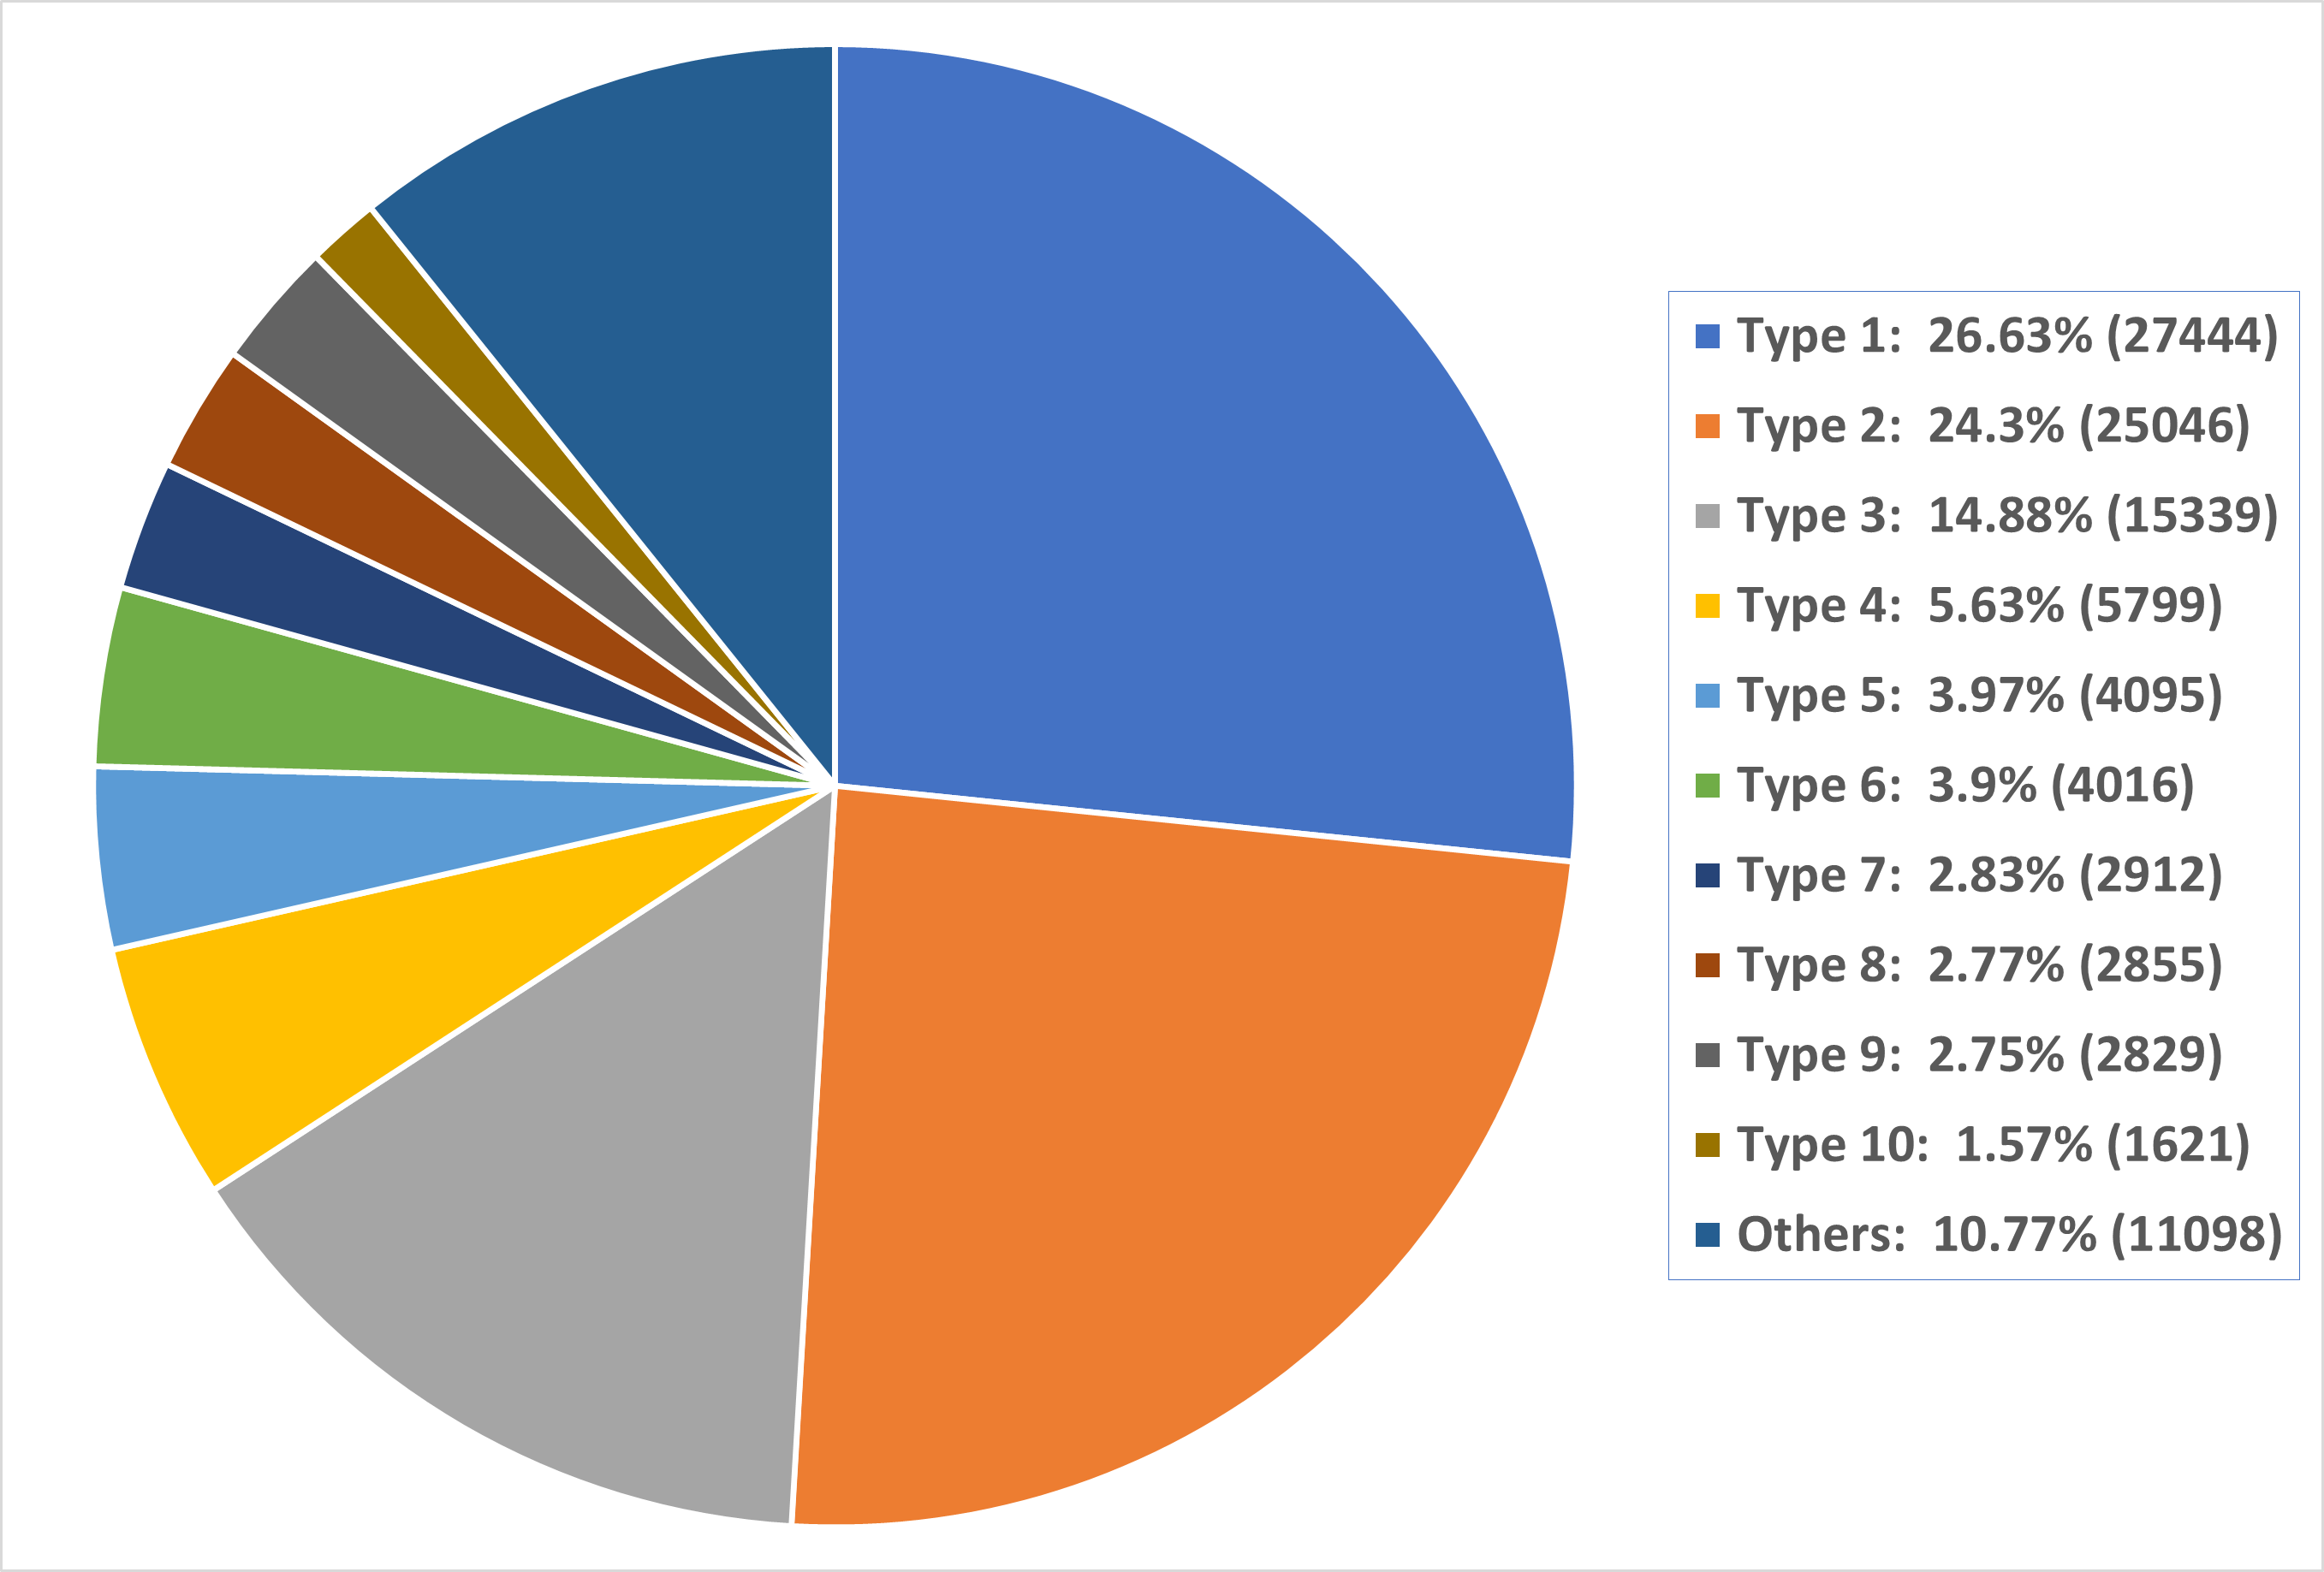
\includegraphics[height=7cm,width=10cm]{images/image1-1.png}
	\caption{ نمودار توزیع انواع تداخلات دارویی }
	\label{image1-1}
	\centering
\end{figure}

با وجود پیشرفت‌های زیادی که در زمینه پیش‌بینی تداخلات دارویی با استفاده از روش‌های مبتنی بر یادگیری ماشین و شبکه‌های عصبی گرافی (\lr{GNN}\LTRfootnote{Graph Neural Network}) صورت گرفته است، همچنان چالش‌های زیادی وجود دارد. یکی از مشکلات عمده، \textbf{کمبود داده‌های برچسب‌گذاری‌شده} برای تداخلات دارویی نادر است. بسیاری از تداخلات دارویی نادر یا کمیاب هستند و از آنجا که این تداخلات در داده‌های آموزشی به‌طور کافی نمایان نشده‌اند، پیش‌بینی آن‌ها با دقت بالا بسیار دشوار است. شکل \ref{image1-1} به خوبی این عدم تعادل در توزیع داده‌های تداخلات دارویی را نشان می‌دهد. سه نوع اول تداخلات دارویی بیش از 65 درصد از کل داده‌ها را تشکیل می‌دهند، در حالی که بسیاری از انواع دیگر تداخلات دارویی سهم بسیار کمی از داده‌ها را به خود اختصاص داده‌اند. این موضوع منجر به \textbf{سوگیری مدل‌ها} می‌شود و موجب می‌گردد که مدل‌ها تنها به تداخلات رایج توجه کرده و در پیش‌بینی تداخلات نادر دقت کمتری داشته باشند \cite{ref_wang2017}.

\subsection{راه‌حل‌های پیشنهادی برای حل محدودیت‌ها}

برای غلبه بر محدودیت‌های موجود در پیش‌بینی تداخلات دارویی و بهبود دقت و کارایی مدل، راه‌حل‌های مختلفی در این پژوهش پیشنهاد و پیاده‌سازی شده است. این راه‌حل‌ها به‌منظور رفع چالش‌هایی نظیر داده‌های نامتوازن، دشواری در تعمیم مدل به داروهای جدید، و بهبود تفسیرپذیری نتایج ارائه شده‌اند.

اولین راه‌حل اساسی در این پژوهش استفاده از معماری چندوجهی است. این معماری به‌منظور مقابله با محدودیت‌های موجود در داده‌ها و پوشش طیف وسیعی از تداخلات دارویی طراحی شده است. در این مدل، از سه نوع داده مختلف استفاده می‌شود که به‌طور همزمان پردازش و ترکیب می‌شوند. ویژگی‌های ساختاری مولکول‌ها با استفاده از شبکه عصبی گرافی پردازش می‌شوند، شباهت‌های دارویی از جنبه‌های مختلف محاسبه می‌شوند، و اطلاعات متنی از منابع علمی با مدل‌های زبانی پیشرفته تحلیل می‌گردند \cite{ref_dai2020}.

برای اطمینان از عملکرد مدل در شرایط مختلف و ارزیابی قابلیت تعمیم آن، سه سناریوی متفاوت برای تقسیم‌بندی داده‌ها به مجموعه‌های آموزش و آزمون طراحی شده است. سناریوی اول از اعتبارسنجی متقاطع استفاده می‌کند که در آن داده‌ها به صورت تصادفی به بخش‌های آموزش و آزمون تقسیم می‌شوند. در سناریوی دوم، برخی داروها به طور کامل از مجموعه آموزش کنار گذاشته شده و فقط در مجموعه آزمون استفاده می‌شوند تا توانایی مدل در تعمیم به داروهای جدید ارزیابی شود. در سناریوی سوم، که چالش‌برانگیزترین حالت است، زوج‌های دارویی کاملاً جدید که هیچ‌کدام از داروهای آن‌ها در مجموعه آموزش حضور نداشته‌اند، برای آزمون مدل استفاده می‌شوند \cite{ref_deng2020}. این سناریوهای مختلف تضمین می‌کنند که مدل در شرایط واقعی و برای پیش‌بینی تداخلات دارویی ناشناخته نیز کارایی لازم را داشته باشد.

یکی دیگر از راه‌حل‌های پیشنهاد شده، بهینه‌سازی پردازش داده‌ها و استفاده از تکنیک‌های پیشرفته یادگیری عمیق است. در بخش پردازش داده‌ها، با هدف بهبود کیفیت پیش‌بینی‌ها و کاهش تأثیر داده‌های نویزدار، فیلترهای کیفیت برای داده‌های ورودی اعمال می‌شود، از تکنیک‌های کاهش ابعاد برای بهبود کارایی محاسباتی استفاده می‌شود، و نرمال‌سازی و استانداردسازی داده‌ها برای بهبود یکنواختی آن‌ها در پیش‌بینی‌ها انجام می‌گردد \cite{ref_he2023}. در بخش یادگیری عمیق نیز، برای افزایش دقت و قابلیت تعمیم مدل، از تکنیک‌های پیشرفته‌ای مانند سازوکار توجه برای پردازش بهینه ساختارهای مولکولی، اشتراک‌گذاری پارامترها برای کاهش پیچیدگی مدل، و تنظیم‌کننده‌ها برای جلوگیری از بیش‌برازش\LTRfootnote{Overfitting} استفاده شده است \cite{ref_li2023}. این اقدامات به مدل کمک می‌کنند تا بهتر و سریع‌تر به یادگیری ویژگی‌های پیچیده پرداخته و عملکرد بهتری از خود نشان دهد.

برای افزایش کاربردپذیری مدل در محیط‌های بالینی، راهکارهایی برای بهبود تفسیرپذیری نتایج نیز ارائه شده است. این راهکارها شامل ارائه وزن‌های اهمیت برای ویژگی‌های مختلف در پیش‌بینی‌ها، نمایش بصری نتایج برای درک بهتر پیش‌بینی‌ها، و ارائه سطح اطمینان برای هر پیش‌بینی می‌باشند \cite{ref_shi2024}. این اقدامات به پزشکان و متخصصان کمک می‌کند تا تصمیمات آگاهانه‌تری در خصوص تجویز داروها بگیرند و از تداخلات دارویی خطرناک پیشگیری کنند.

با پیاده‌سازی این راه‌حل‌ها، مدل پیشنهادی توانایی غلبه بر محدودیت‌های موجود را خواهد داشت و می‌تواند عملکرد قابل‌قبولی در پیش‌بینی تداخلات دارویی از خود نشان دهد.

\section{ساختار پایان‌نامه}

این پایان‌نامه در پنج فصل اصلی سازماندهی شده است. فصل اول با عنوان مقدمه، به معرفی پیش‌زمینه و اهمیت موضوع تداخلات دارویی می‌پردازد و در آن دامنه و محدودیت‌های پژوهش و راه‌حل‌های پیشنهادی ارائه شده‌اند. فصل دوم به بررسی مفاهیم اساسی در حوزه تداخلات دارویی و مرور پژوهش‌های پیشین اختصاص دارد. در این فصل روش‌های موجود برای شناسایی تداخلات دارویی، کاربرد یادگیری ماشین در این حوزه و شکاف‌های تحقیقاتی موجود مورد بحث قرار گرفته‌اند. در فصل سوم، جزئیات مدل پیشنهادی تشریح شده است که شامل معماری مدل، نحوه جمع‌آوری و پیش‌پردازش داده‌ها و جزئیات پیاده‌سازی مدل می‌باشد. فصل چهارم به ارزیابی جامع مدل پیشنهادی می‌پردازد که شامل معرفی سناریوهای ارزیابی، ارائه نتایج مدل در هر سناریو و مقایسه با روش‌های موجود است. این فصل همچنین به تفسیر نتایج و تحلیل عملکرد مدل از منظر کاربردی در محیط‌های بالینی می‌پردازد. در فصل پایانی، خلاصه‌ای از یافته‌های اصلی پژوهش و دستاوردهای آن ارائه شده است و پیشنهاداتی برای ادامه این مسیر تحقیقاتی در کارهای آینده مطرح شده‌اند.

علاوه بر فصول اصلی، این پایان‌نامه شامل سه پیوست است که در پیوست الف توضیح کامل 65 نوع تداخل دارویی مورد بررسی، در پیوست ب معیارهای ارزیابی و روش‌های محاسبه آن‌ها، و در پیوست ج واژه‌نامه معادل‌های فارسی اصطلاحات تخصصی ارائه شده است.
